\documentclass{sigchi-ext}
% Please be sure that you have the dependencies (i.e., additional
% LaTeX packages) to compile this example.
\usepackage[T1]{fontenc}
\usepackage{textcomp}
\usepackage[scaled=.92]{helvet} % for proper fonts
\usepackage{graphicx} % for EPS use the graphics package instead
\usepackage{balance}  % for useful for balancing the last columns
\usepackage{booktabs} % for pretty table rules
\usepackage{ccicons}  % for Creative Commons citation icons
\usepackage{ragged2e} % for tighter hyphenation

% Some optional stuff you might like/need.
% \usepackage{marginnote} 
% \usepackage[shortlabels]{enumitem}
% \usepackage{paralist}
% \usepackage[utf8]{inputenc} % for a UTF8 editor only

%% EXAMPLE BEGIN -- HOW TO OVERRIDE THE DEFAULT COPYRIGHT STRIP --
% \copyrightinfo{Permission to make digital or hard copies of all or
% part of this work for personal or classroom use is granted without
% fee provided that copies are not made or distributed for profit or
% commercial advantage and that copies bear this notice and the full
% citation on the first page. Copyrights for components of this work
% owned by others than ACM must be honored. Abstracting with credit is
% permitted. To copy otherwise, or republish, to post on servers or to
% redistribute to lists, requires prior specific permission and/or a
% fee. Request permissions from permissions@acm.org.\\
% {\emph{CHI'14}}, April 26--May 1, 2014, Toronto, Canada. \\
% Copyright \copyright~2014 ACM ISBN/14/04...\$15.00. \\
% DOI string from ACM form confirmation}
%% EXAMPLE END

% Paper metadata (use plain text, for PDF inclusion and later
% re-using, if desired).  Use \emtpyauthor when submitting for review
% so you remain anonymous.
\def\plaintitle{MagicMirror - An Interactive Drawing Surface for Public Areas} \def\plainauthor{First Author, Second Author, Third Author,
  Fourth Author, Fifth Author, Sixth Author}
\def\emptyauthor{}
\def\plainkeywords{Authors' choice; of terms; separated; by
  semicolons; include commas, within terms only; required.}
\def\plaingeneralterms{Documentation, Standardization}

\title{MagicMirror - An Interactive Drawing Surface for Public Areas}

\numberofauthors{4}
% Notice how author names are alternately typesetted to appear ordered
% in 2-column format; i.e., the first 4 autors on the first column and
% the other 4 auhors on the second column. Actually, it's up to you to
% strictly adhere to this author notation.
\author{%
  \alignauthor{%
    \textbf{First Author}\\
    \affaddr{University of Author} \\
    \affaddr{Authortown, CA 94022, USA} \\
    \email{author1@anotherco.edu} }\alignauthor{%
    \textbf{Fifth Author}\\
    \affaddr{YetAuthorCo, Inc.}\\
    \affaddr{Authortown, BC V6M 22P Canada}\\
    \email{author5@anotherco.com} } \vfil \alignauthor{%
    \textbf{Second Author}\\
    \affaddr{VP, Authoring}\\
    \affaddr{Authorship Holdings, Ltd.}\\
    \affaddr{Awdur SA22 8PP, UK}\\
    \email{author2@author.ac.uk} }\alignauthor{%
    \textbf{Sixth Author}\\
    \affaddr{Universit\'e de Auteur-Sud}\\
    \affaddr{40222 Auteur France}\\
    \email{author6@author.fr} } \vfil \alignauthor{%
    \textbf{Third Author}\\
    \textbf{Fourth Author}\\    
    \affaddr{L\={e}khaka Interaction Labs}\\
    \affaddr{Bengaluru 560 080, India}\\
    \email{author3@anotherco.com} \\
    \email{author4@hchi.anotherco.com} }\alignauthor{%
    \textbf{Seventh Author}\\
    \affaddr{Department of Skrywer}\\
    \affaddr{University of Umbhali}\\
    \affaddr{Cape Town, South Africa}\\
    \email{author7@umbhaliu.ac.za} } }

% Make sure hyperref comes last of your loaded packages, to give it a
% fighting chance of not being over-written, since its job is to
% redefine many LaTeX commands.
\definecolor{linkColor}{RGB}{6,125,233}
\hypersetup{%
  pdftitle={\plaintitle},
%  pdfauthor={\plainauthor},
  pdfauthor={\emptyauthor},
  pdfkeywords={\plainkeywords},
  bookmarksnumbered,
  pdfstartview={FitH},
  colorlinks,
  citecolor=black,
  filecolor=black,
  linkcolor=black,
  urlcolor=linkColor,
  breaklinks=true,
}

% \reversemarginpar%

\begin{document}

%% For the camera ready, use the commands provided by the ACM in the Permission Release Form.
%\CopyrightYear{2007}
%\setcopyright{rightsretained}
%\conferenceinfo{WOODSTOCK}{'97 El Paso, Texas USA}
%\isbn{0-12345-67-8/90/01}
%\doi{http://dx.doi.org/10.1145/2858036.2858119}
%% Then override the default copyright message with the \acmcopyright command.
%\copyrightinfo{\acmcopyright}

\maketitle

% Uncomment to disable hyphenation (not recommended)
% https://twitter.com/anjirokhan/status/546046683331973120
\RaggedRight{} 

% Do not change the page size or page settings.
\begin{abstract}
\justify
People have been using surfaces to spread the information years ago. We would like to inherit the that social concept. Therefore, we develop MagicMirror, a reflective drawing surface integrating with motion technology, allowing people to pass messages by using finger. Finally, we also would like to test the humans reactions towards MagicMirror to suggest improvements for future developments.
\end{abstract}

\keywords{reflective surface, collaborative surface, drawing, magic mirror}

\category{H.5.3}{Group and Organization Interfaces}{Group Interface, Collaborative Interface}

\bibliographystyle{SIGCHI-Reference-Format}
\section{Introduction}
\justify
Communication refers to the process of passing messages between peoples which may be verbal, non - verbal or visual ~cite{noauthor_3_nodate}. This is a collaborative process, which makes people more social and interactive. Ages ago, as a form of visual communication, people used to carve messages on stone pillars to communicate very well across time which is perfect for the common areas ~\cite{noauthor_history_nodate}. This paper focuses on this same concept integrated with the technology using the mirror, a reflective surface.

Over the past couple of decades, growing technology has revolutionised the world. This is constantly having a massive impact on the human race at every stage of societal development. Not only computers connected objects and sensors are getting smarter but also any object around us and the way we interact with an emerging world is getting smarter and more enhanced ~\cite{noauthor_technology_2018}. We picked a mirror as our interaction device and made it smarter with additional technologies. We merged the concept of passing messages with mirror so we call it ''Magic Mirror''. So far, no smart mirror has been developed that makes the mirror more appealing to general users. Also, none of the smart mirrors developed has the concept of social communication. This paper suggests a new mode of passing messages which connects people that underlie social interaction.

''Passing Messages'' is a primary goal of Magic Mirror. Sharing the message just with the reflective mirror using hand gestures without any additional devices or IoT, just makes it so simple to use. One of the purposes of this concept is making people more social not just by sharing messages but also this lets the multiple participants work together to create something which is obviously a team building.

\section{Related Work}
The proposed Magic Mirror represents a social and collaborative interaction interface that provides a platform to share the message with the personal or group contribution. And there has been number of projects based on the smart mirror which are related and driven in similar direction. Philips Homelab is a permanent fully functional home laboratory built to study how people interact with interactive and automated home environment ~\cite{noauthor_philips_2008}. Smart Lighting system, augmented broadcasts, smart music collection, smart memory browsing system, interactive mirror are some of the setups in homelab. Interactive mirror can be placed in room or washroom and can be personalized according to the need of the end user. Every person can customise the content (i.e. cartoons for children's, adults can get live news feeds and updates on weathers, traffics, mail etc) ~\cite{henk_hagenbeuk_homelab:_nodate}.

Researchers from Griffith University conducted the early exploration of the suitability of Leap Motion controller in the project entitled ''The Leap Motion controller: A view on sign language''. They conducted this research for Auslan (Australian Sign Language) and they found out the leap motion to be perfect for basic signs but not appropriate for complex signs ~\cite{potter_leap_2013}.

Another project named FitMirror as carried out by students of Ulm University. They created a fitmirror system to help users to get up in the morning and get motivated for the day. They built the recognition system for fun and normal exercises which made the exercise fun for even middle and low motivated persons. They used Kinect for emotion recognition and hand trace for different games ~\cite{besserer_fitmirror:_2016}.

In comparison, to various projects and works mentioned above, our proposed aim is different which is to develop social interaction between people by sharing messages using the combined functionality of mirror and leap motion.


\section{Case Study}
We would like to show the features of our product and with some users evaluate our product and get feedback from the users for future improvement.
\subsection{Problem Statement}
We would like to investigate 2 hypothesis:
\begin{itemize}
	\item[H1] People are more motivated to draw on a surface with some drawing on it
	\item[H2] People are more motivated to draw when they are in a small group.
\end{itemize}

\subsection{Prototype}
Based on the model of House and Hill 1997 ~\cite{houde_chapter_1997}, we develop both "Role" and "Look and feel" prototype to test the research question of our concern. We intend to provide both an overview of the functionality and concrete experience successively via each prototype.
For the "Role" prototype, we use "Role Playing" as an internal development. It helps the team members to share the same understanding of the MagicMirror concept and to get a feeling how the basic functionalites work.

Regarding "Look and feel" prototype, we build a mirror surface. To get a reflection of a user like a mirror does, reflection sol firm having around 80\% of reflection was used in front of 21- inch monitor. Interaction between user and the system was done using leap motion. Leap motion detects the air gesture or finger movement as input without any direct contact with the surface. The graphics editor Tux Paint was used for the drawing interface. The leap motion SDK was used to make leap motion work on windows platform as Windows 10 was used as the environment to work for Tux Paint. Users can draw on MagicMirror surface using the finger movement without touching it.
\begin{figure}[h]
	\center
  	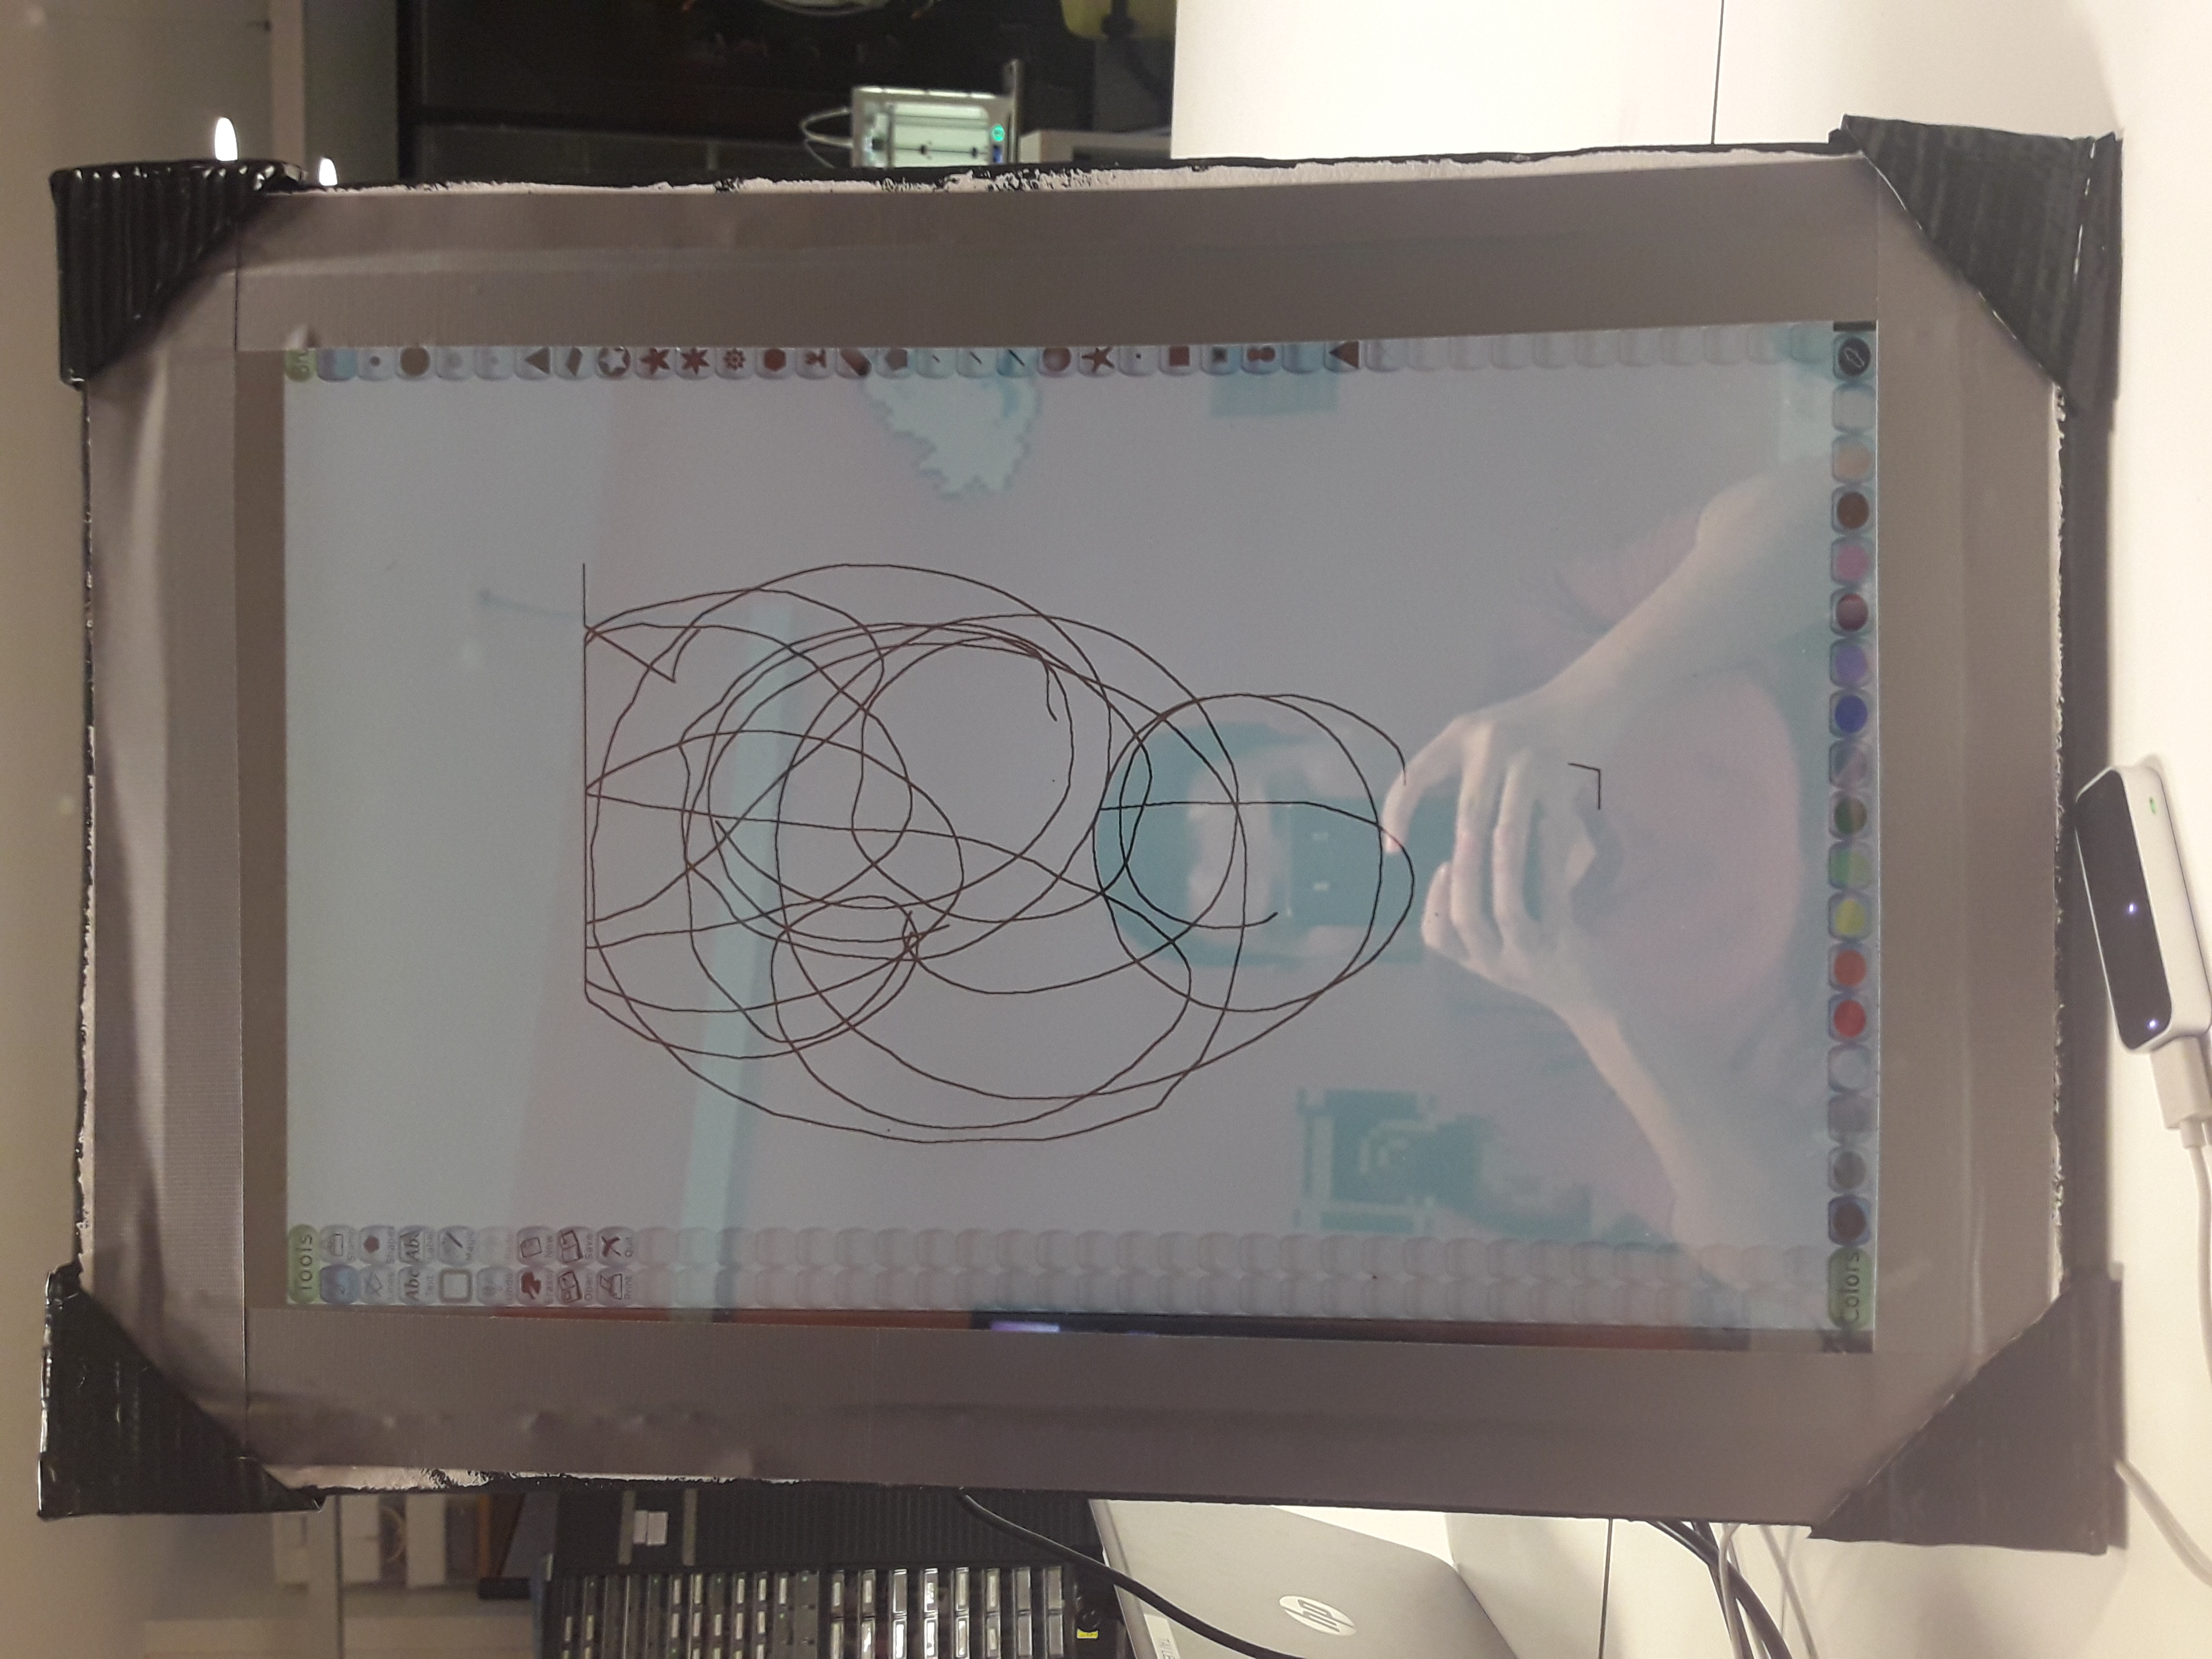
\includegraphics[height=4cm, scale=0.2]{images/prototype}
	\caption{User using the MagicMirror}
	\center
  	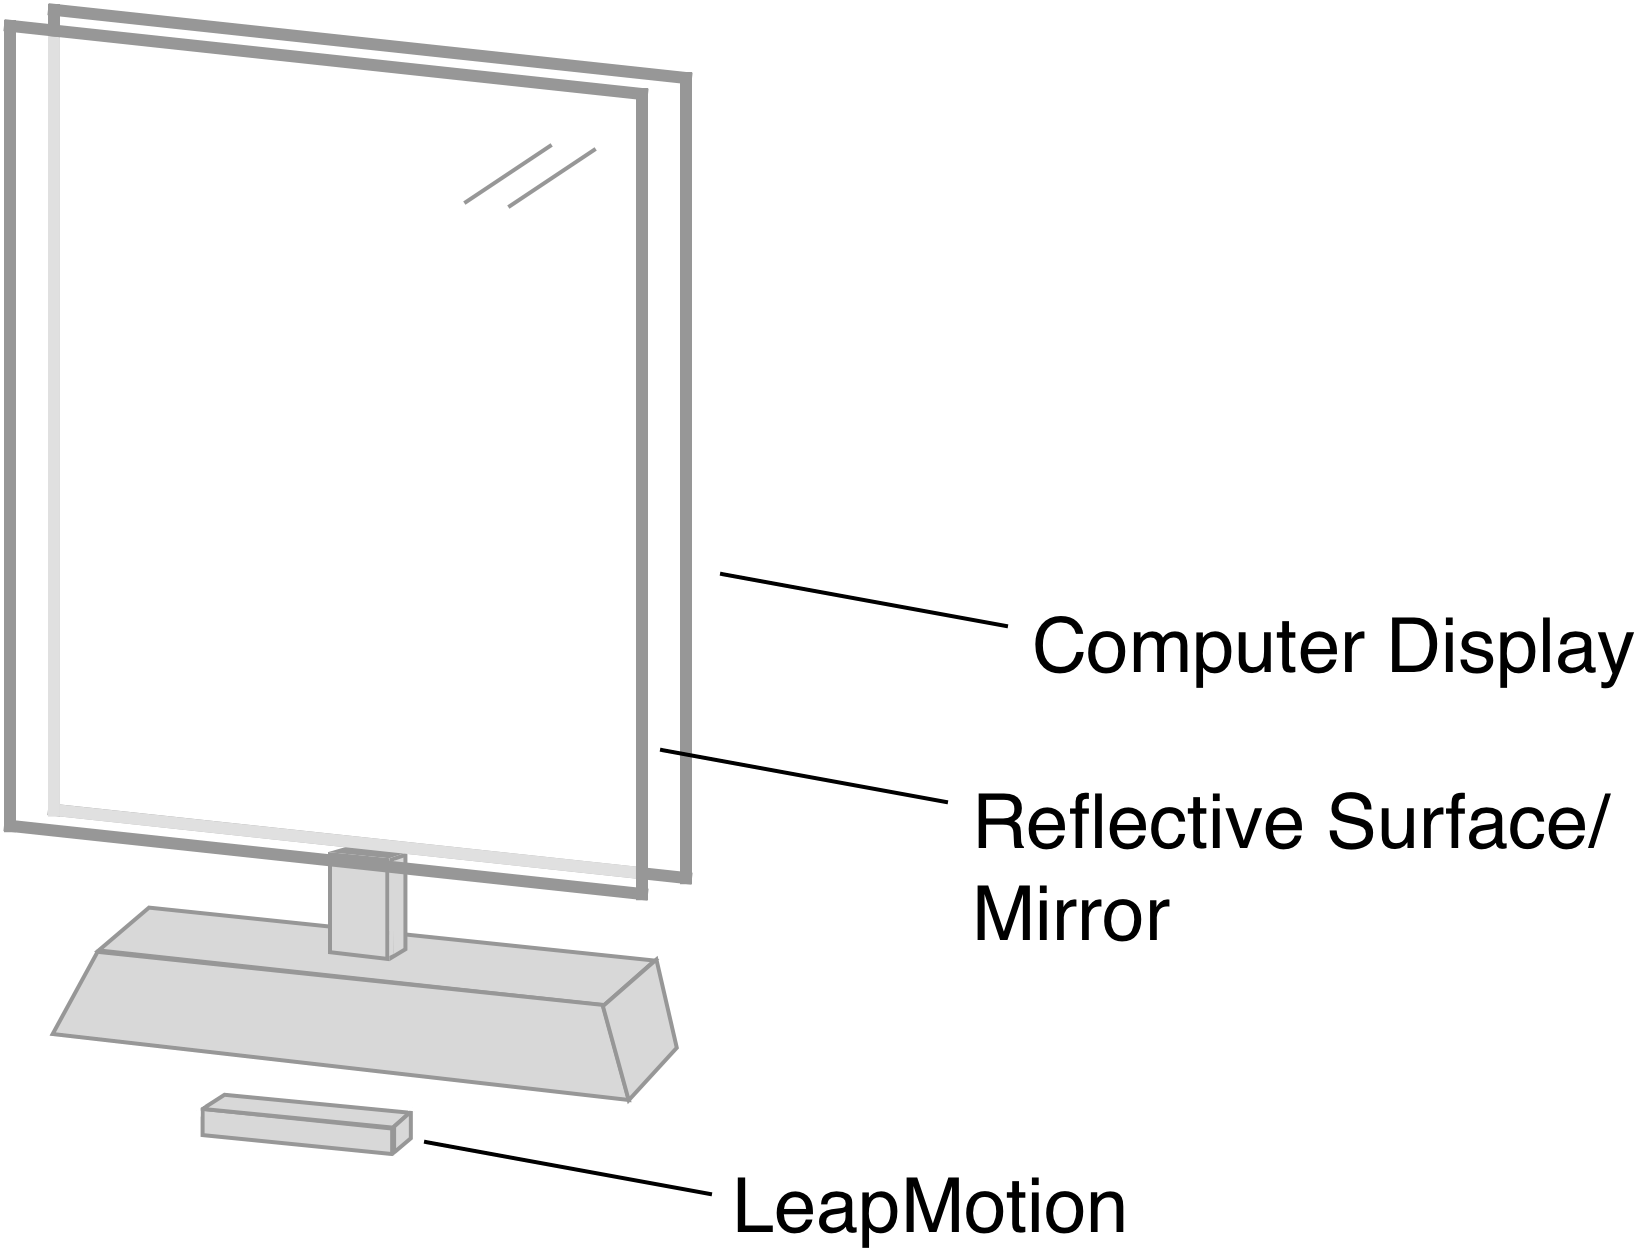
\includegraphics[height=4cm, scale=0.5]{images/cartoon}
  	\caption{The components of MagicMirror}
  
\end{figure}

\textit{Hardware}
A glass with reflection solar film (80\% reflection surface), a Leap Motion, a 21" LCD.
\textit{Software}
Touchless for Windows an Leap Motion application developed by Leap Motion Gallery, Tux Paint.


\subsection{Deployment/Methods}
Deployment is the process of using the developed system to an effective action. In this section the complete deployment of the MagicMirror is described.
The user should stand in front of mirror in the range of leap motion and point one finger in the mirror then starts drawing.
After the whole setup, we used two different environments for testing our prototype i.e. Controlled environment and Natural environment.

In Controlled environment the testing of the prototype was done by individuals or people in a small group which were invited by us. The MagicMirror was deployed in the makerspace. For controlled environment, there were also two testcase. First case is that when the mirror was blank and the second one was when there was already some previous drawings in the mirror. The main motive of controlled environment testing was to test the usability testing. There were 24 users invited as an individual and 11 users in a group of 2 or 3. All the users invited were the student of Hi\O  and they have to answer the questionnaire. The questionnaire is mainly to rate how enjoyable the product is and how motivated the user were to use the prototype. They need to give the answer in form rating. The rating is from 1 (not at all) to 5 (very enjoyable/motivated).
 
Similarly, the MagicMirror was deployed in the hallway in front of the cafeteria in the University for Natural environment. The hallway was chosen as it is used almost by all students and staff of all faculties. Therefore, we have a wider range of participants. The main motive of the natural testing was to gain the attention of the random people passing the hallway to do field studies, to observe how the people interact with the mirror without any prior information. We did not count the exact number of participants involved in this testing as we only want to observe how user interact with the MagicMirror generally.

\section{Early Results}
The questionnaire was not able to show a difference in motivation depending on the initial state of the mirror. Therefore, we reject our H1 hypothesis. Our second hypothesis H2 is accepted. Even though the average amount of enjoyment is only slightly higher for people in a small group, the difference between the min and max value shows that people in a small group enjoy it more.

The observations mainly showed two points we will declare in the following. 

 Firstly, people stop to look at the mirror. During our observations, people who were not alone stopped more often than persons who were alone. We could also observe that people who walked in the direction of the cafeteria also stopped for a longer time than the person who was walking towards the classrooms. This might be due to the lack of time when people have to go to classes.

Secondly, people left quickly when the mirror did not work the expected way. We could clearly see that people had their difficulties with drawing and writing in the air with one finger. It might be that for people it is not intuitive to write something without touching the surface the person want to write on.

Besides the results from the questionnaire, it was also noticable during the observations, people who started testing the prototype with a non-blank surface, asked for a new blank surface if the previous drawing occupied more than \textasciitilde20\% of the surface. Due to the small given surface, the surface was most of the time too full after the use of one person/group.

\section{Future Work}
\bibliography{ref2}

\end{document}

%%% Local Variables:
%%% mode: latex
%%% TeX-master: t
%%% End:
